\begin{frame}
  \frametitle{Experimental setup}
  \begin{itemize}
  \item[-] Kuka FRI Joint specific impedance control mode
    \begin{itemize}
    \item[] $\boldsymbol{\tau}_{cmd} = K_j(\vec{q}_{FRI} - \vec{q}_{msr}) + D(d_{j}) + \boldsymbol{\tau}_{FRI} + \vec{f}_{dynamics}(\vec{q}, \dot{\vec{q}}, \ddot{\vec{q}})$
    \end{itemize}
  \item[-] $K_j = 0$
  \item[-] $\vec{q}_{FRI} = \vec{q}_{msr}$
  \item[-] $d_{j} = 0$
  \item[-] $\vec{f}_{dynamics}(\vec{q}, \dot{\vec{q}}, \ddot{\vec{q}})$ supposed to be $\vec{G}(\vec{q})$
  \item[-] $\boldsymbol{\tau}_{FRI}$ used as commanded torque
  \end{itemize}
\end{frame}

\begin{frame}
  \frametitle{Experimental setup}
  \framesubtitle{Issues}
  \begin{flalign*}
    &\boldsymbol{\tau}_{FRI} = C \dot{\vec{q}} +  B\vec{a}_{app}(\vec{\dot{q}})\\
    &\boldsymbol{\tau}_{FRI} = C \dot{\vec{q}} + J^{T}_{F} ( B_A \vec{a}_{hic}(\vec{w}_{F}, \dot{\vec{q}}) - B_A \dot{J_{A,E}} \vec{\dot{q}} + \vec{w}_{F}) + \boldsymbol{\tau}_{null}(J_{a_{4}})
  \end{flalign*}
  
  \begin{itemize}
    \item[-] masses, inertias and CoM of links are not exact:
      \begin{itemize}
      \item[-] $B$ given by FRI {\color{dgreen}\cmark}
      \item[-] $C \dot{\vec{q}}$ neglected {\color{red}\xmark}
      \end{itemize}
      
      \item[-] only $\vec{q}$ is available
      \begin{itemize}
      \item[-] $\dot{\vec{q}}$ estimated using an exponential smoothing {\color{orange}\cmark}
      \end{itemize}
        
    \item[-] Jacobians are evalutated using KDL library {\color{dgreen}\cmark} 

    \item[-] $\vec{w}_F$ given by force/torque sensor
      \begin{itemize}
      \item[-] $\vec{w}_F = \vec{w}_{ideal} + \vec{w}_{offs}$ (offset not yet estimated) {\color{red}\xmark}
      \item[-] problems with light sensitivity! {\color{dgreen}\cmark}
    \end{itemize}
    \item[-] friction not compensated in control laws {\color{red}\xmark}
  \end{itemize}
\end{frame}

\begin{frame}
  \frametitle{Experimental setup}
  \framesubtitle{Approaching phase}
  \begin{itemize}
  \item[-] initial configuration: $\begin{bmatrix} -0.91 & 0.24 & 0.24 & 2.21 & 0.36 &-2.90 \end{bmatrix}$
  \item[-] final configuration: $\begin{bmatrix} -0.7 & 0.04 & 0.16 & 2.96 & 0.11 &-2.69 \end{bmatrix}$
  \item[-] duration $5$s
  \item[-] $K_p = \mathrm{diag}(1600)$
  \item[-] $K_d = \mathrm{diag}(30)$
  \end{itemize}
\end{frame}

\begin{frame}
  \frametitle{Experimental setup}
  \framesubtitle{Approaching phase - Results}
  \begin{center}
   \vskip-0.1in
    \begin{tabular}{cc}
      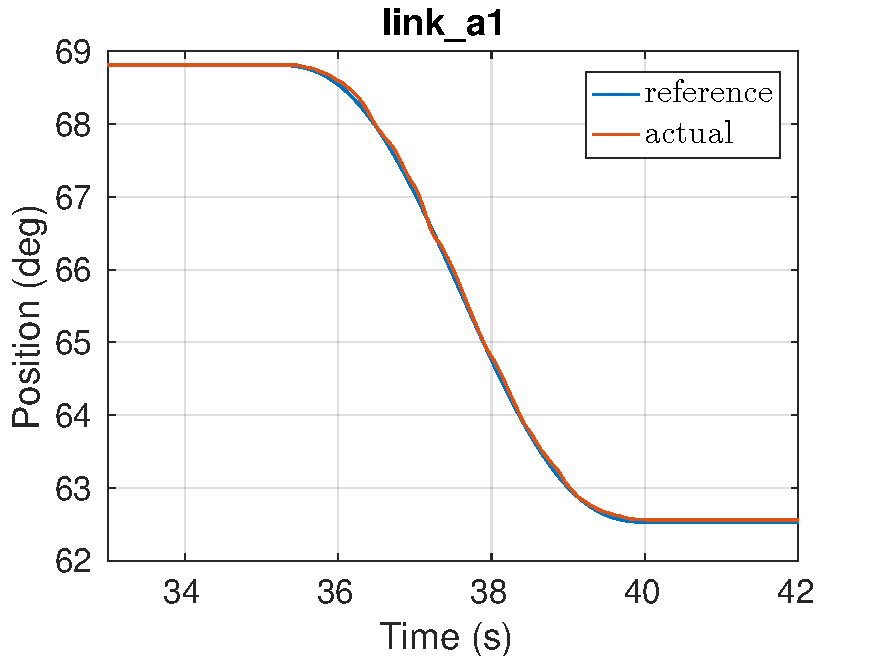
\includegraphics[scale=0.34]{cart_real_3_a1} &
      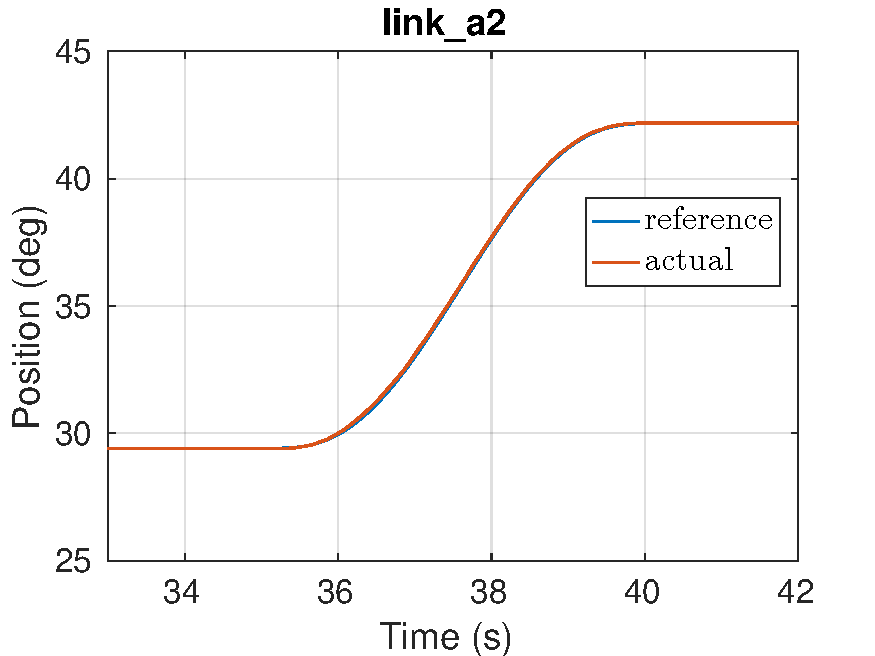
\includegraphics[scale=0.34]{cart_real_3_a2}
    \end{tabular}
  \end{center}
  \begin{center}
   \vskip-0.1in
    \begin{tabular}{cc}
      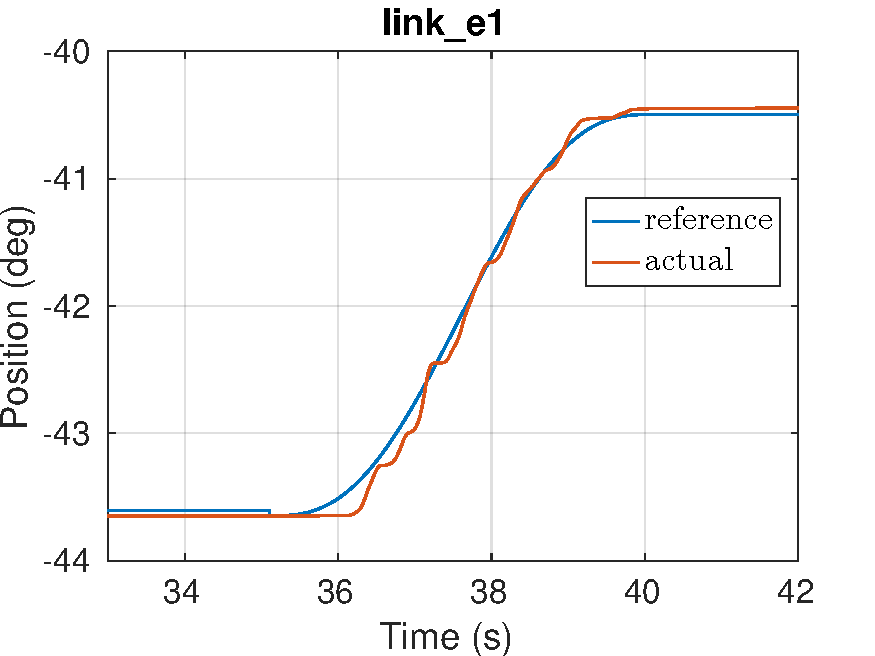
\includegraphics[scale=0.34]{cart_real_3_e1} &
      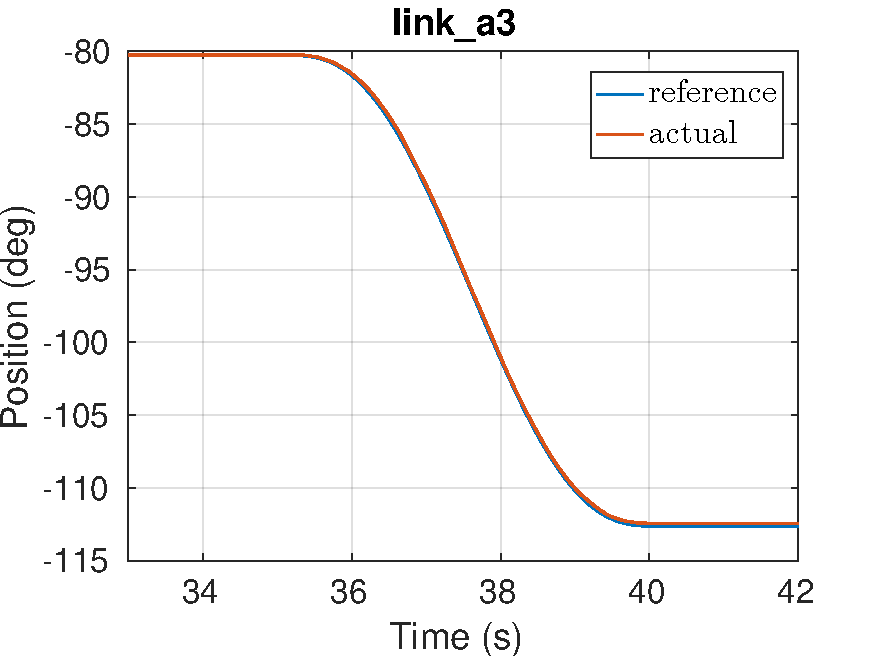
\includegraphics[scale=0.34]{cart_real_3_a3}
    \end{tabular}
  \end{center}
\end{frame}

\begin{frame}
  \frametitle{Experimental setup}
  \framesubtitle{Approaching phase - Results}
  \begin{center}
   \vskip-0.1in
    \begin{tabular}{cc}
      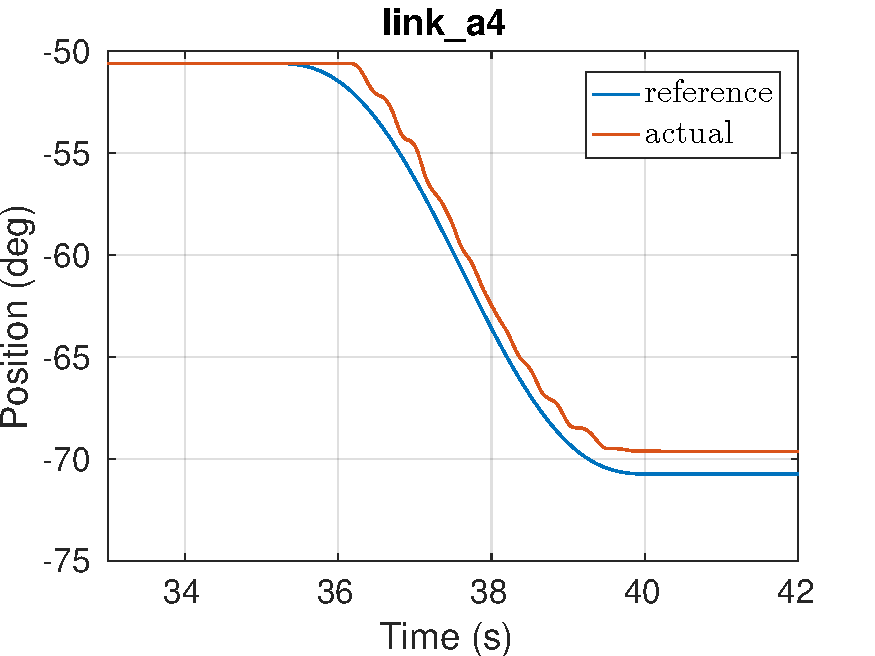
\includegraphics[scale=0.34]{cart_real_3_a4} &
      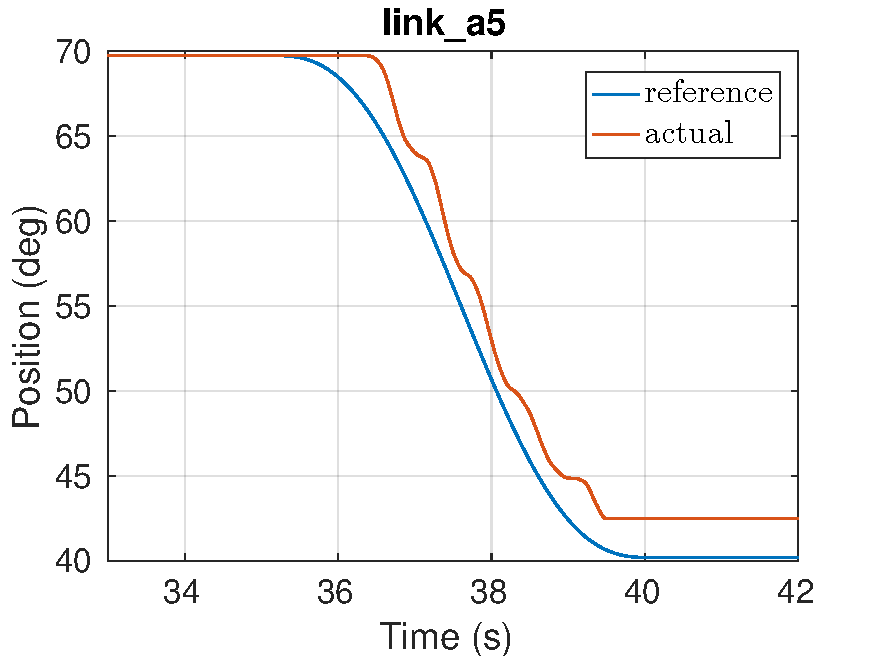
\includegraphics[scale=0.34]{cart_real_3_a5}
    \end{tabular}
  \end{center}
  \begin{center}
   \vskip-0.1in
    \begin{tabular}{c}
      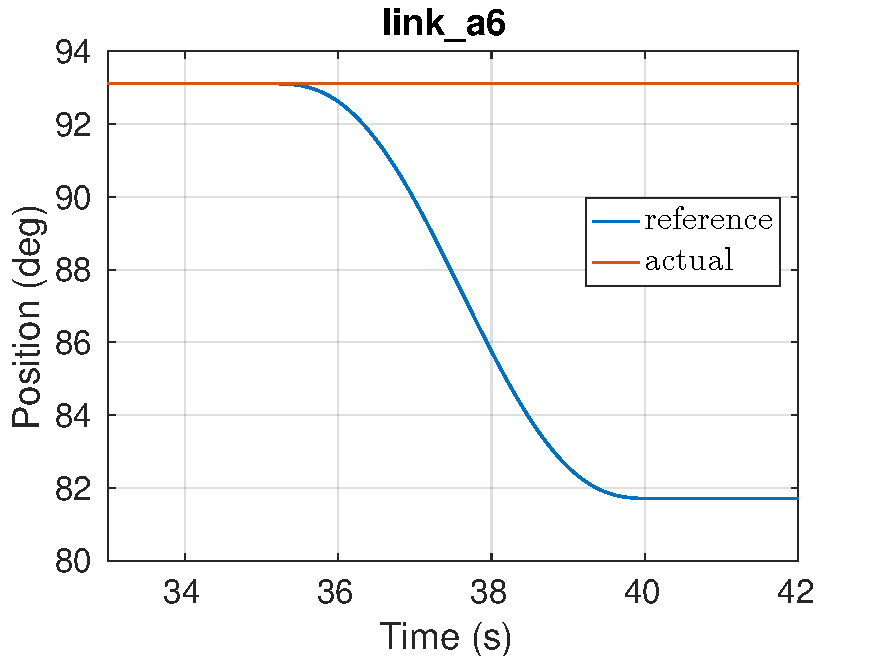
\includegraphics[scale=0.34]{cart_real_3_a6}
    \end{tabular}
  \end{center}
\end{frame}

\begin{frame}
  \frametitle{Experimental setup}
  \framesubtitle{Force regulation}
  \begin{itemize}
  \item[-] duration $2$s
  \item[-] $K_p = \mathrm{diag}(300)$
  \item[-] $K_d = \mathrm{diag}(30)$
  \item[-] $b_f = 25$
  \end{itemize}
\end{frame}

\begin{frame}
  \frametitle{Experimental setup}
  \framesubtitle{Force regulation - Results ($k_{f} = 1$)}
  \begin{center}
   \vskip-0.1in
    \begin{tabular}{ccc}
      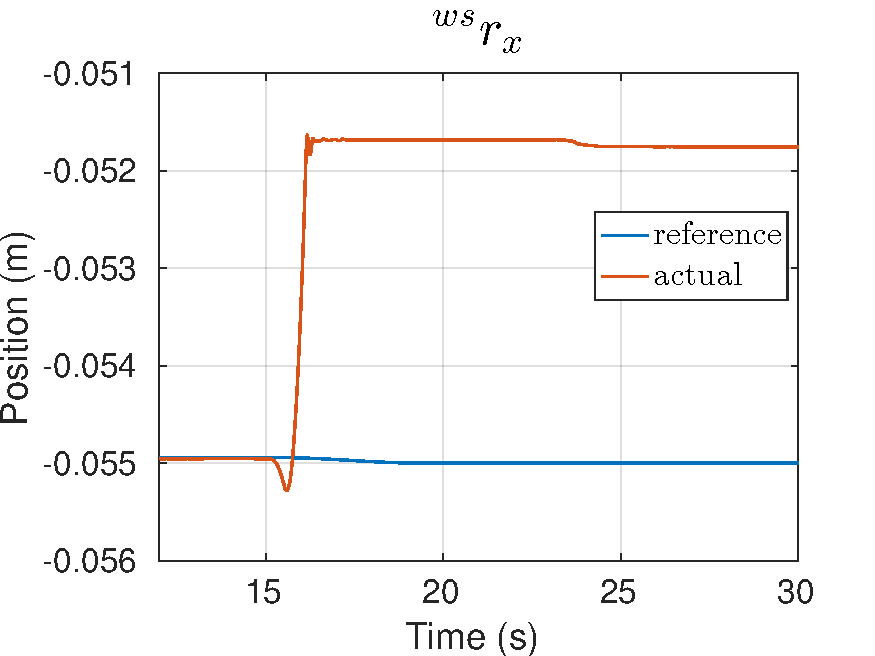
\includegraphics[scale=0.26]{force_real_13_x} &
      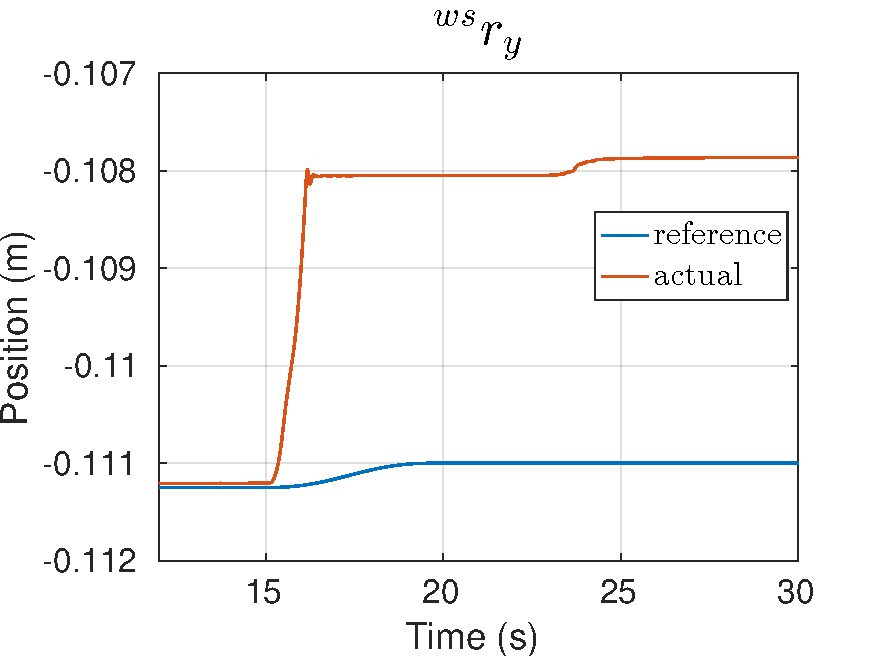
\includegraphics[scale=0.26]{force_real_13_y} &
      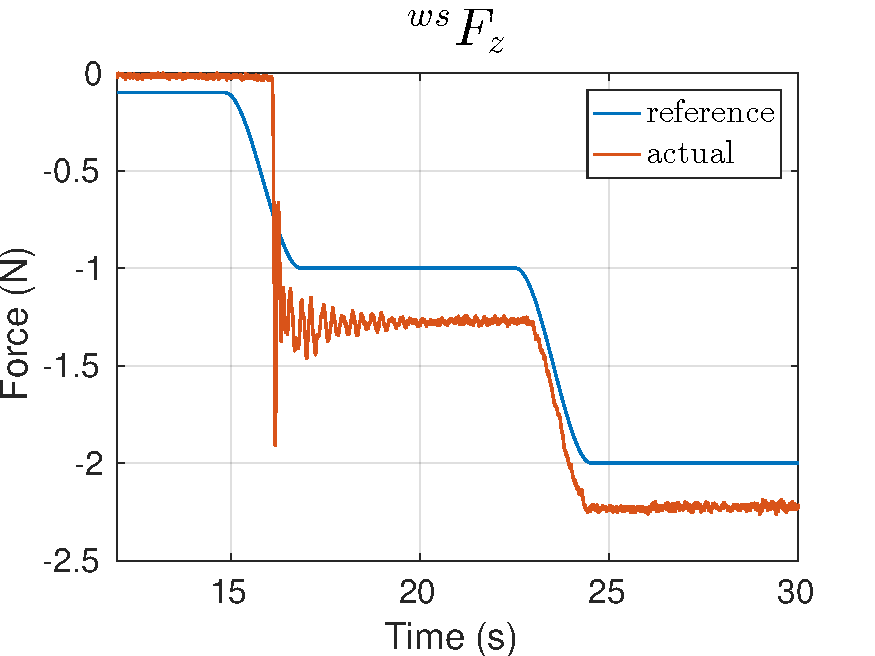
\includegraphics[scale=0.26]{force_real_13_z} \\
      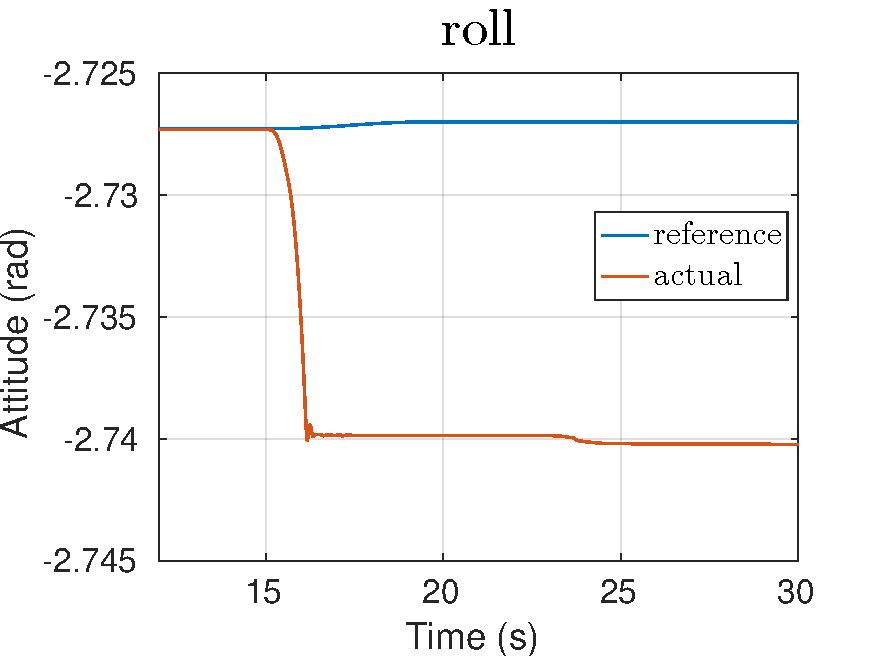
\includegraphics[scale=0.26]{force_real_13_roll} &
      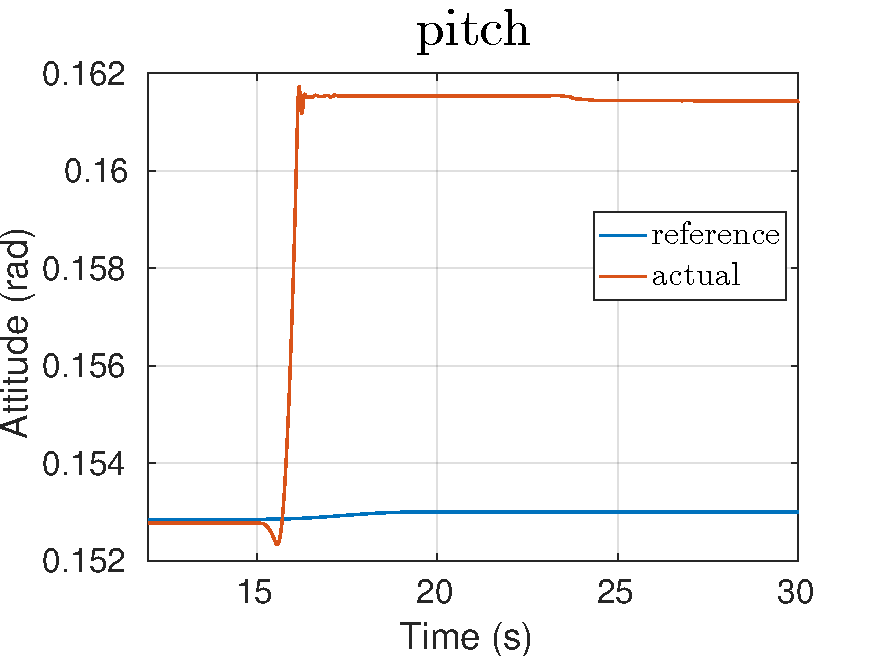
\includegraphics[scale=0.26]{force_real_13_pitch} &
      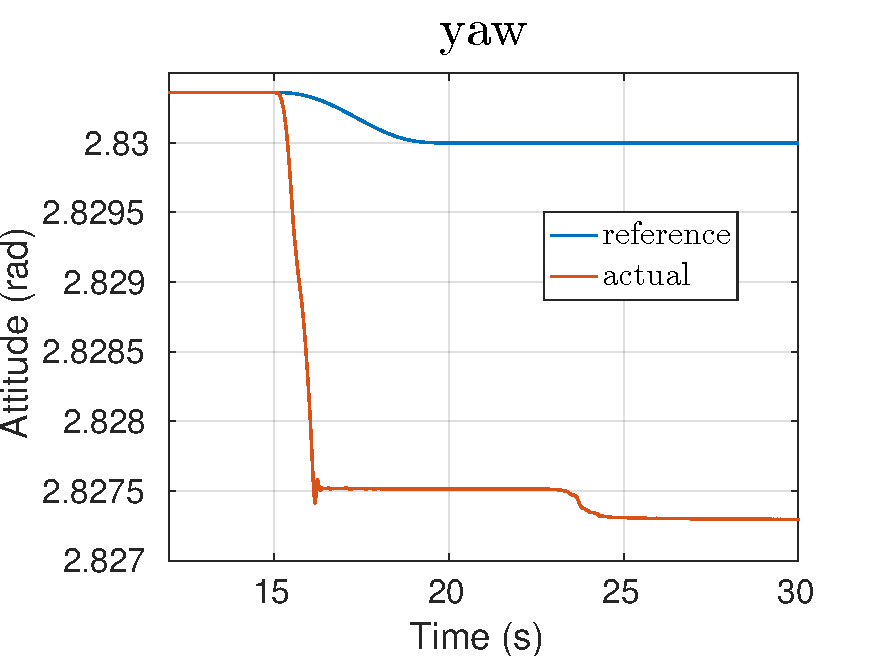
\includegraphics[scale=0.26]{force_real_13_yaw}
    \end{tabular}
  \end{center}
\end{frame}

\begin{frame}
  \frametitle{Experimental setup}
  \framesubtitle{Force regulation - Results ($k_{f} = 1.5$)}
  \begin{center}
   \vskip-0.1in
    \begin{tabular}{ccc}
      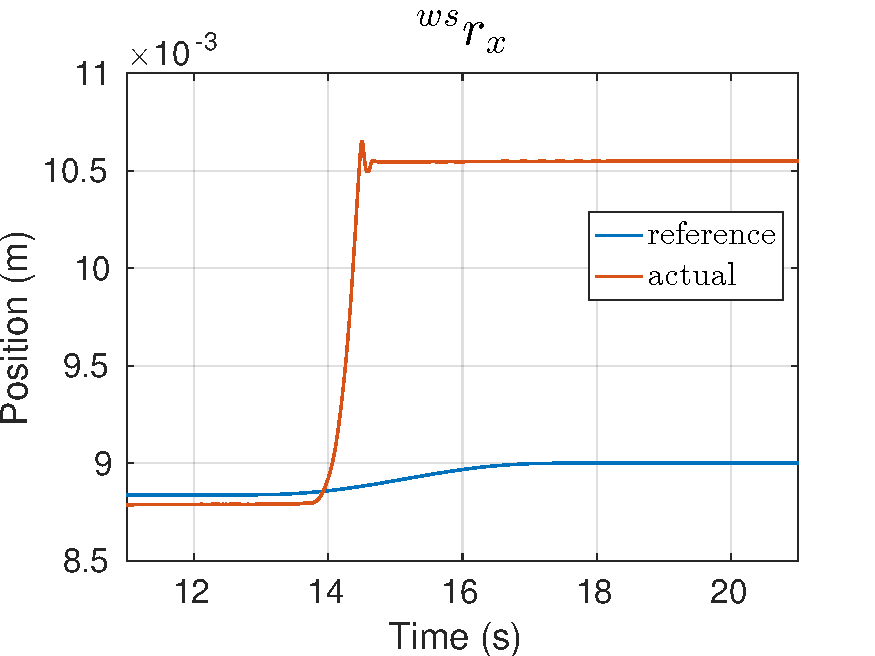
\includegraphics[scale=0.26]{force_real_16_x} &
      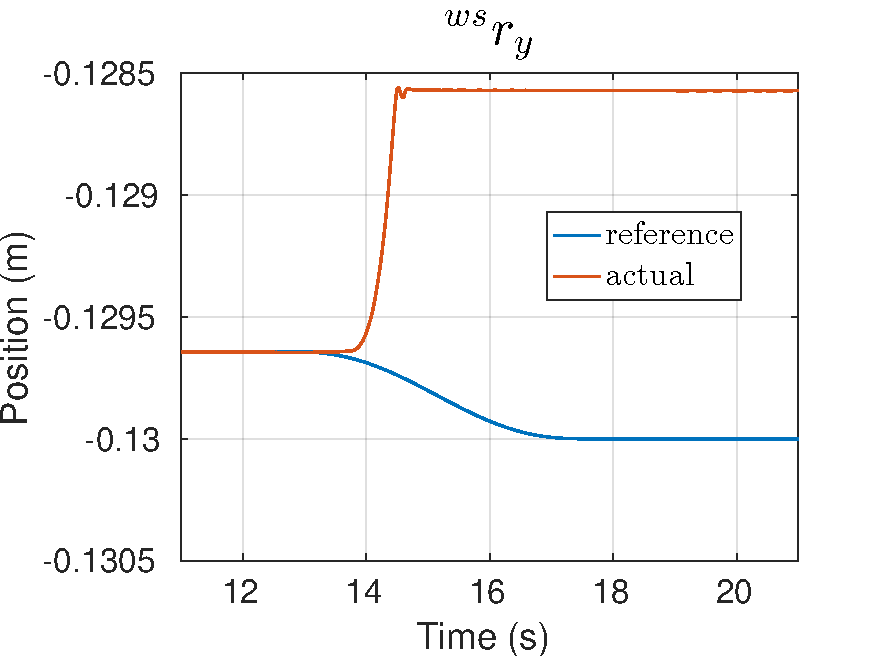
\includegraphics[scale=0.26]{force_real_16_y} &
      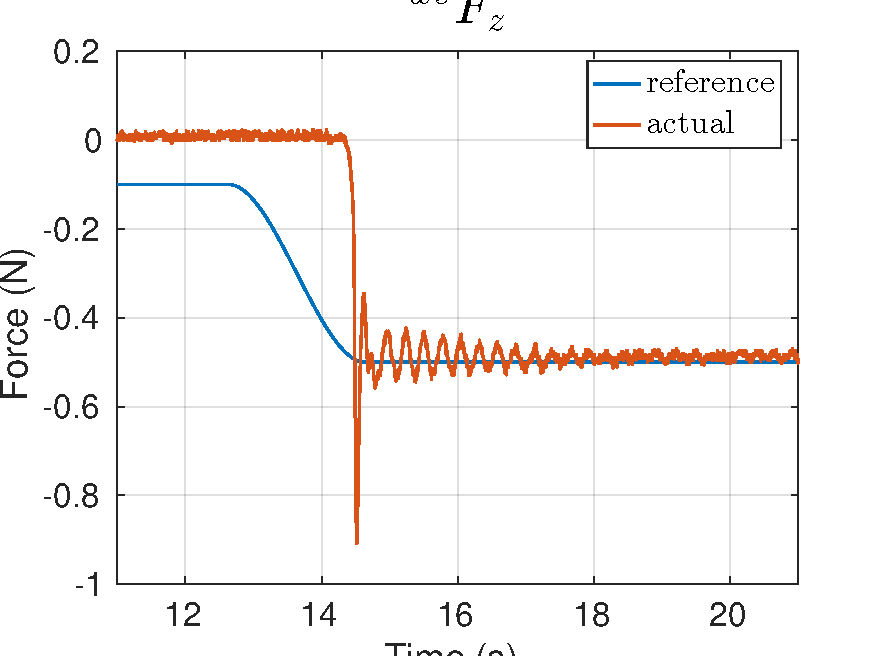
\includegraphics[scale=0.26]{force_real_16_z} \\
      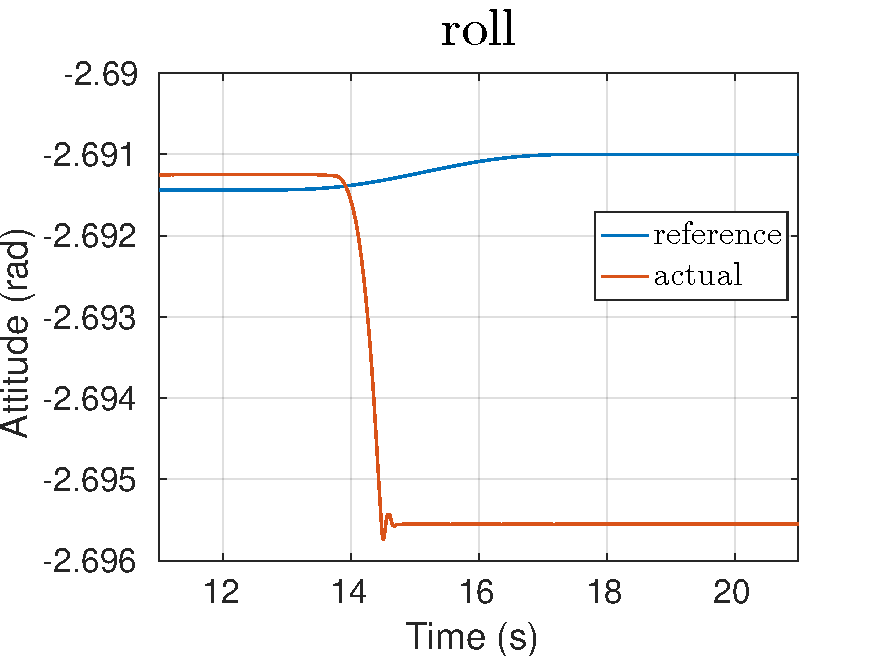
\includegraphics[scale=0.26]{force_real_16_roll} &
      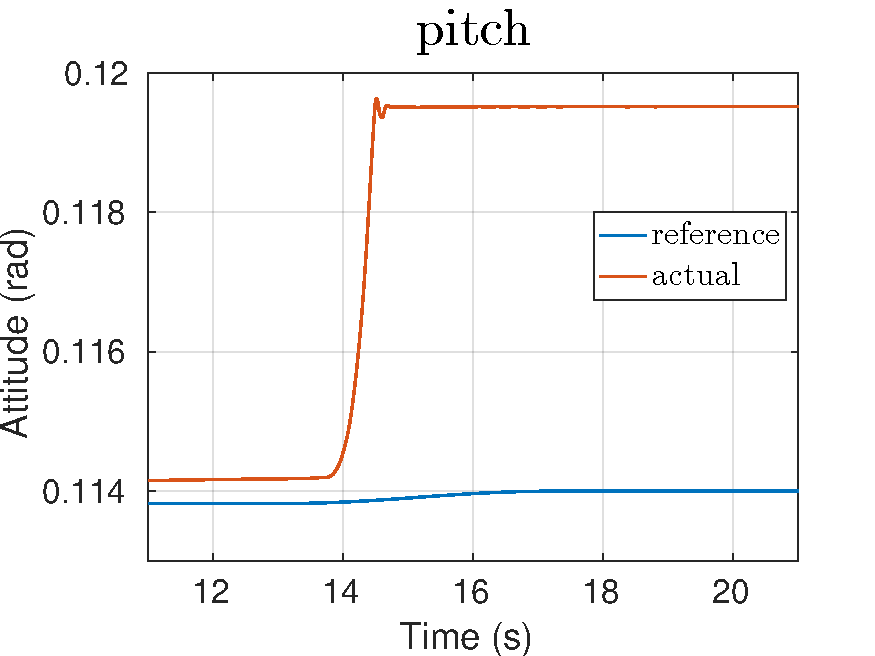
\includegraphics[scale=0.26]{force_real_16_pitch} &
      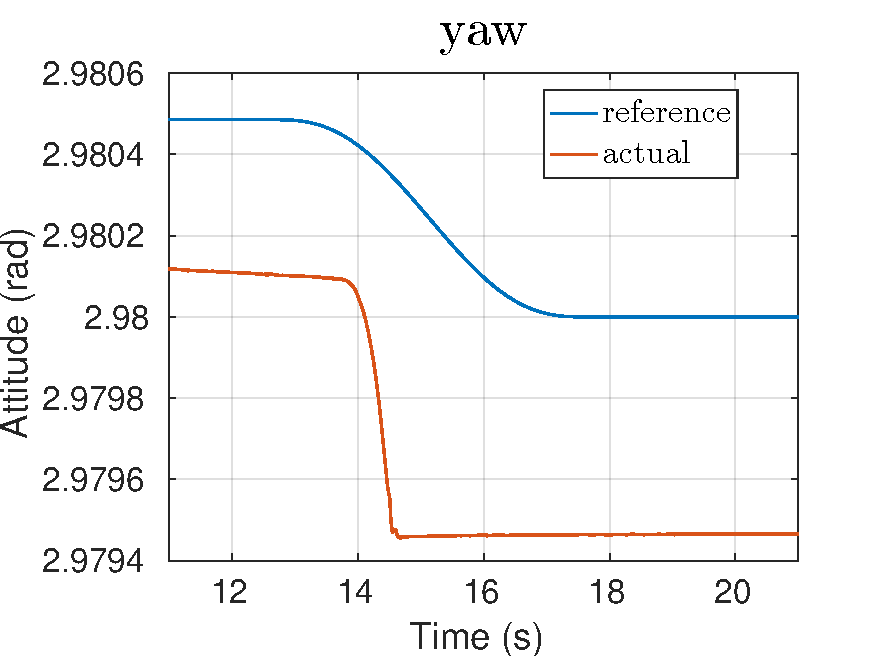
\includegraphics[scale=0.26]{force_real_16_yaw}
    \end{tabular}
  \end{center}
\end{frame}

\begin{frame}
  \frametitle{Experimental setup}
  \framesubtitle{Force regulation + motion}
  \begin{itemize}
  \item[-] reference trajectory duration $5$s
  \item[-] reference force duration $2$s
  \item[-] $K_p = \mathrm{diag}(300)$
  \item[-] $K_d = \mathrm{diag}(30)$
  \item[-] $k_{f} = 1.5$
  \item[-] $b_f = 25$
  \end{itemize}
\end{frame}

\begin{frame}
  \frametitle{Experimental setup}
  \framesubtitle{Force regulation + motion - Results}
  \begin{center}
   \vskip-0.1in
    \begin{tabular}{ccc}
      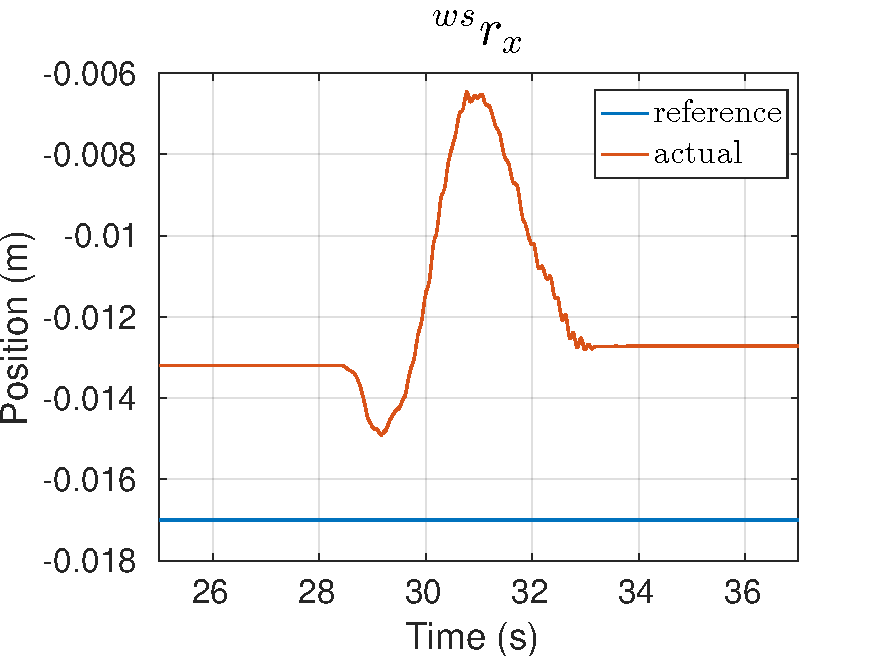
\includegraphics[scale=0.26]{force_real_11_x} &
      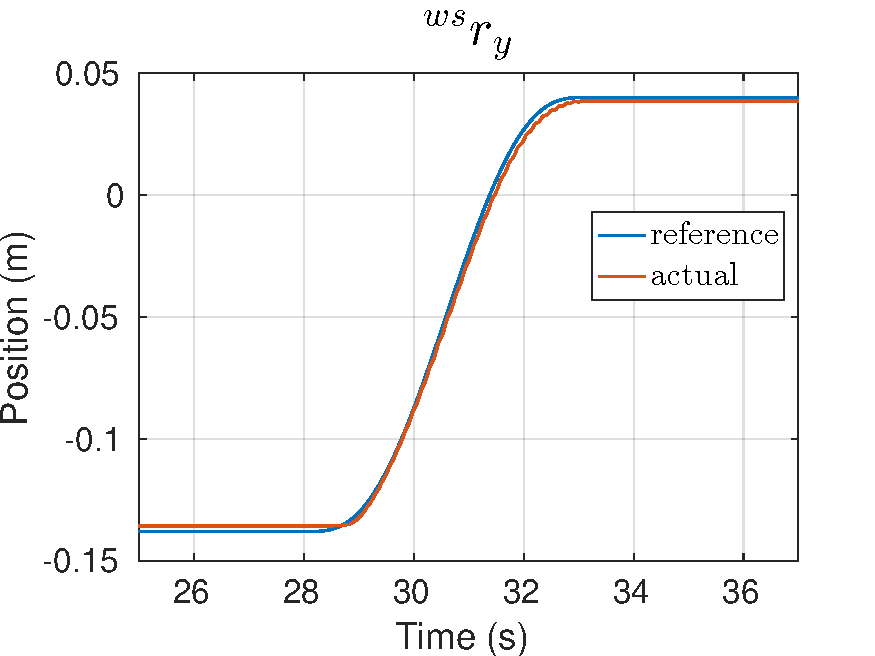
\includegraphics[scale=0.26]{force_real_11_y} &
      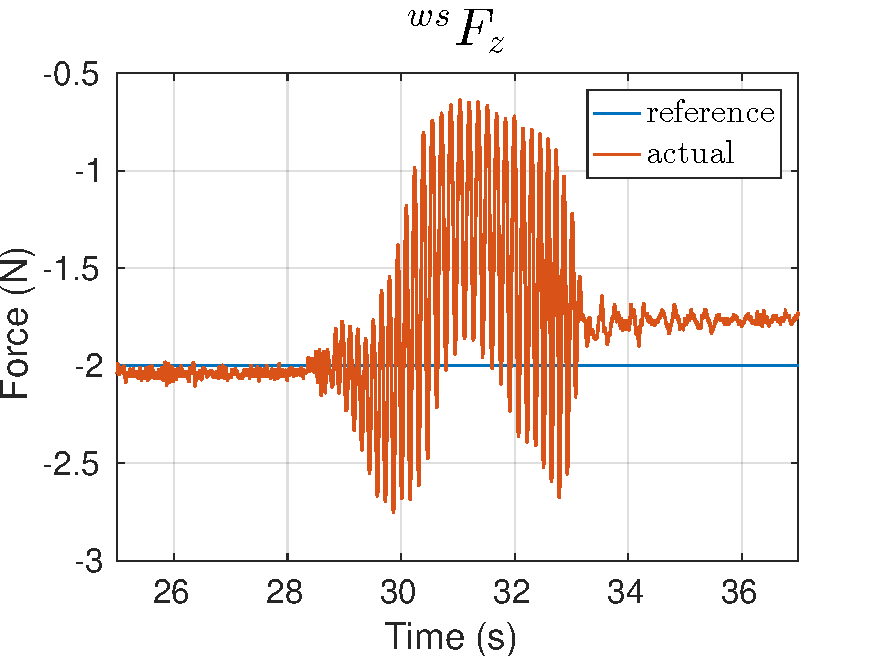
\includegraphics[scale=0.26]{force_real_11_z} \\
      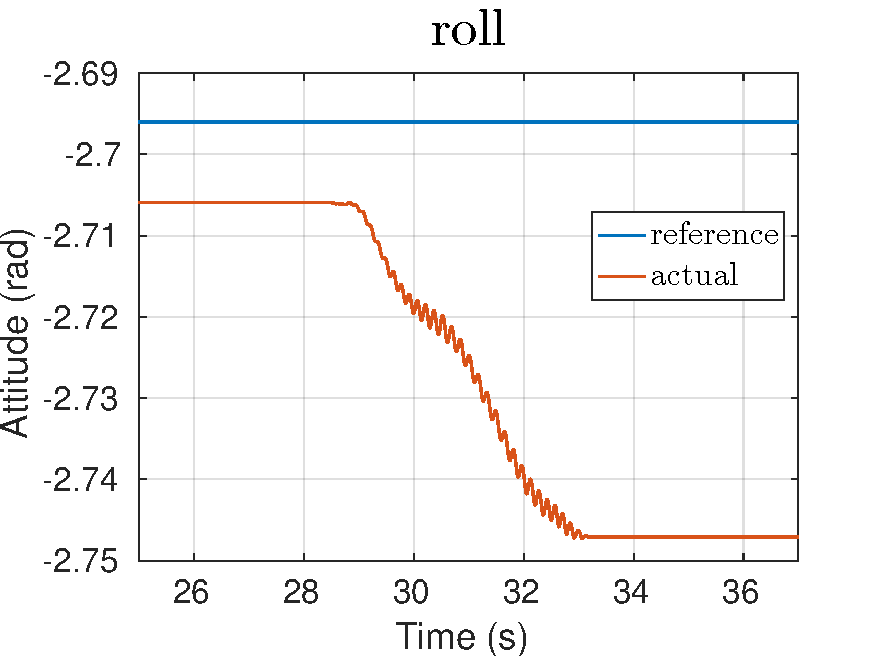
\includegraphics[scale=0.26]{force_real_11_roll} &
      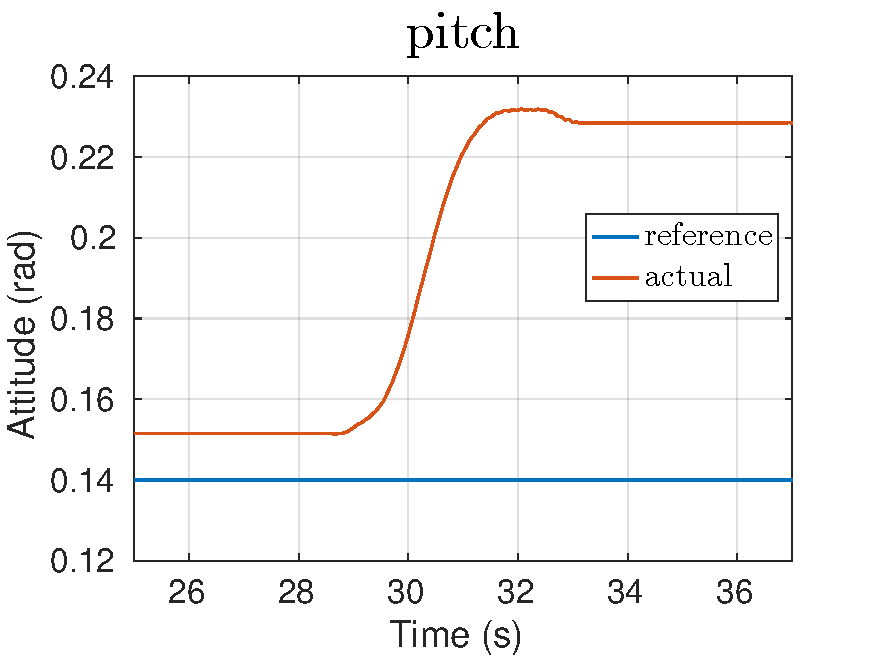
\includegraphics[scale=0.26]{force_real_11_pitch} &
      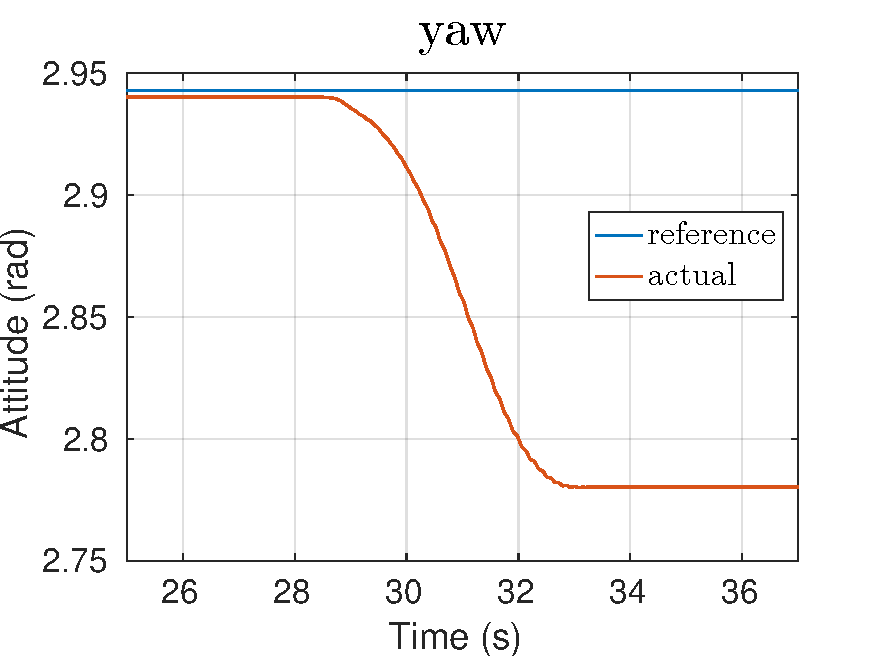
\includegraphics[scale=0.26]{force_real_11_yaw}
    \end{tabular}
  \end{center}
\end{frame}

\begin{frame}
  \frametitle{Experimental setup}
  \framesubtitle{Force regulation + motion - Results}
  \begin{center}
   \vskip-0.1in
    \begin{tabular}{ccc}
      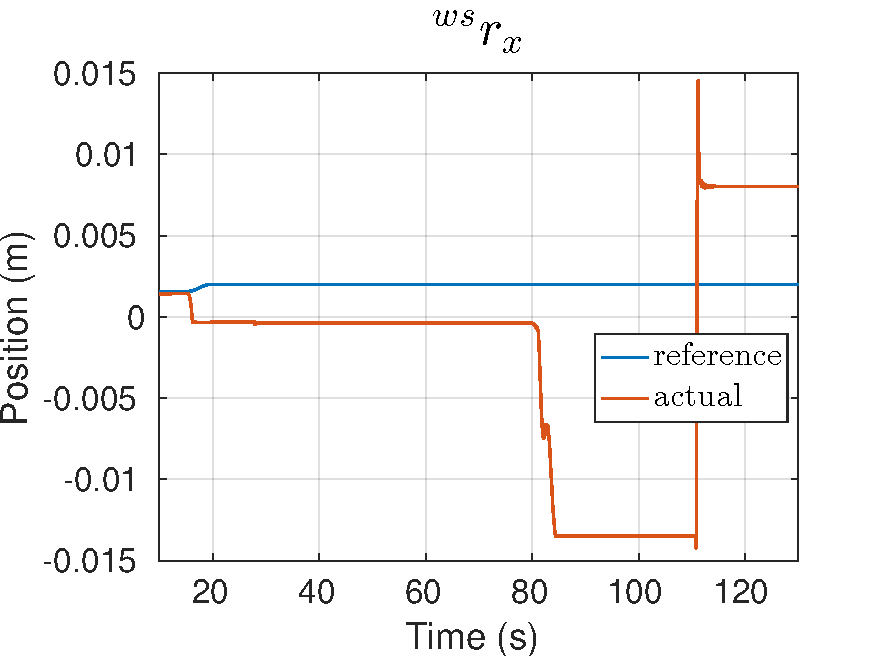
\includegraphics[scale=0.26]{force_real_10_x} &
      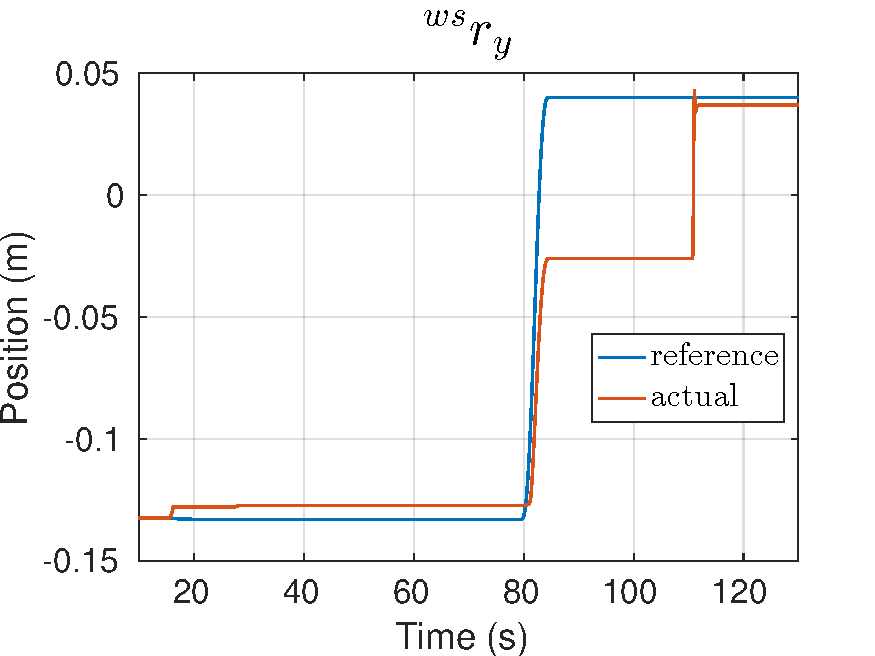
\includegraphics[scale=0.26]{force_real_10_y} &
      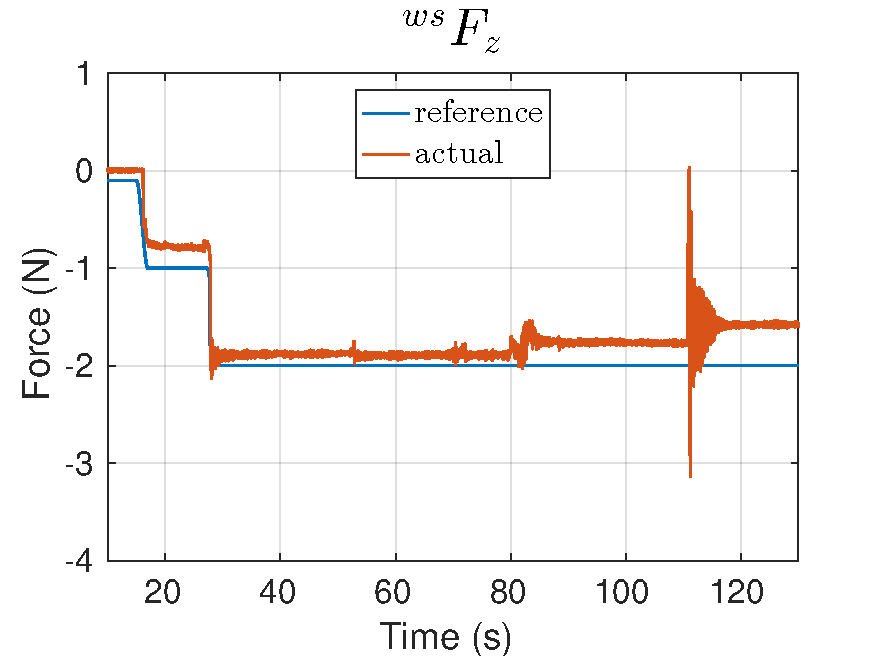
\includegraphics[scale=0.26]{force_real_10_z} \\
      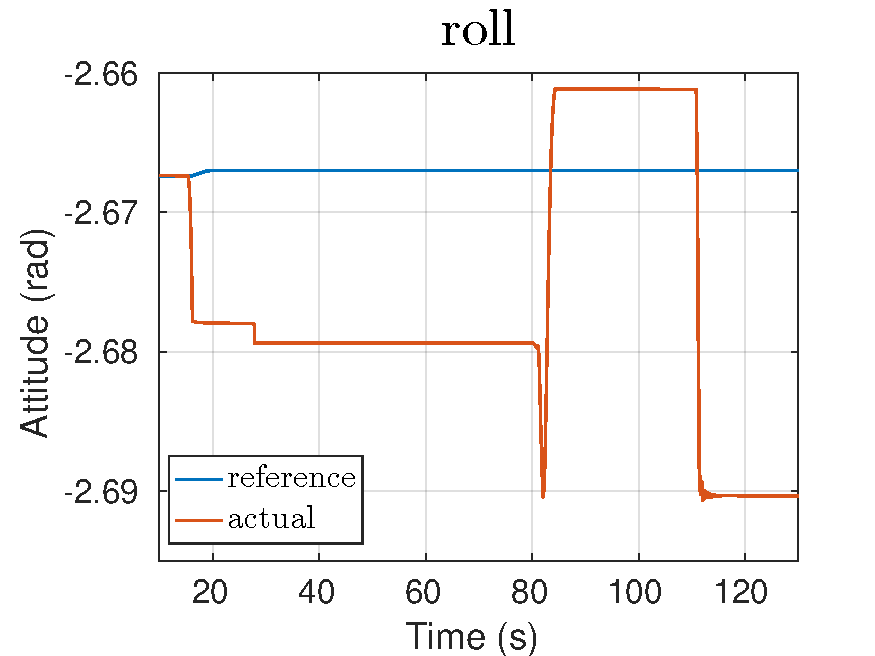
\includegraphics[scale=0.26]{force_real_10_roll} &
      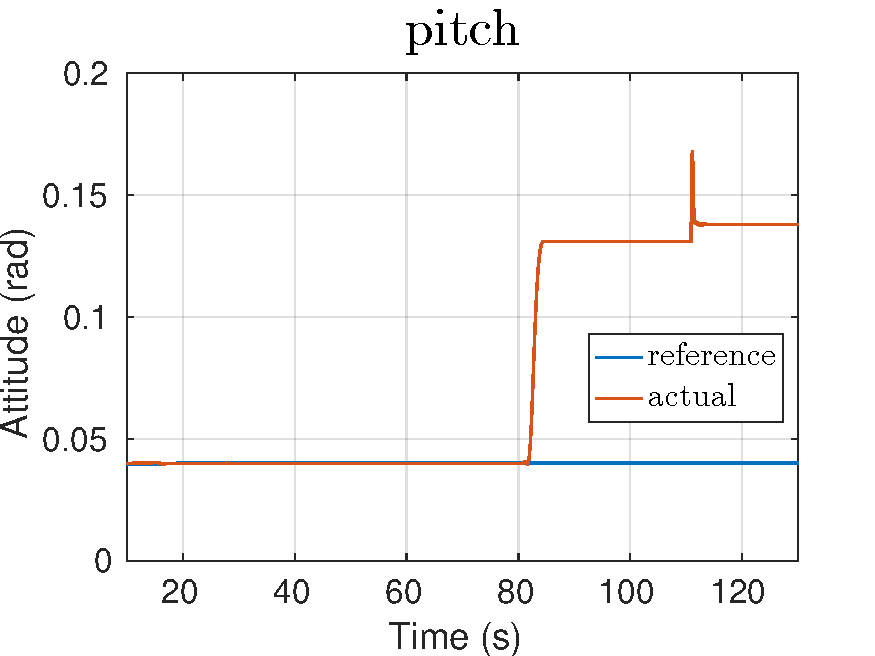
\includegraphics[scale=0.26]{force_real_10_pitch} &
      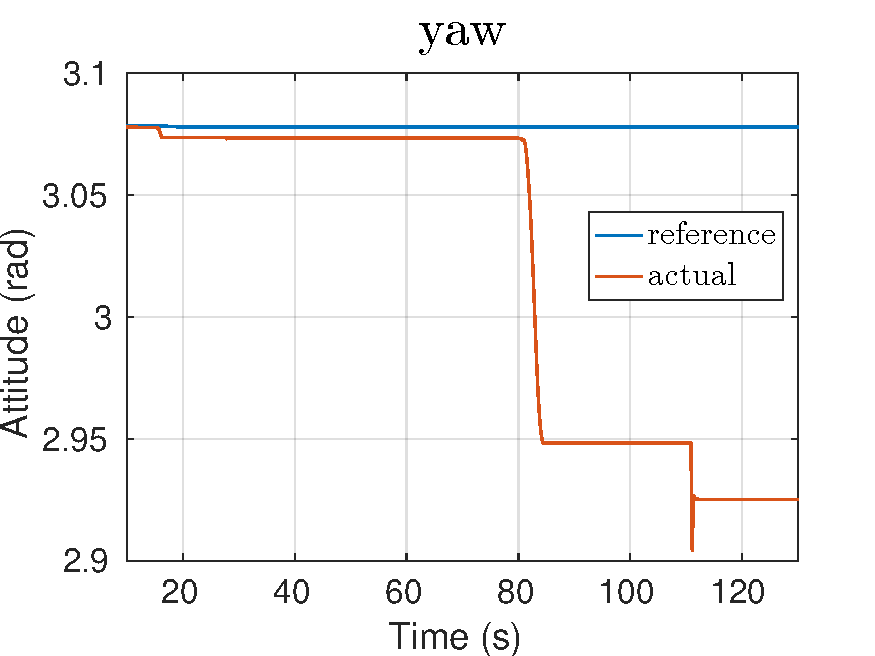
\includegraphics[scale=0.26]{force_real_10_yaw}
    \end{tabular}
  \end{center}
\end{frame}
